% !TeX spellcheck = pt_BR

%%%%%%%%%%%%%%%%%%%%%%%%%%%%%%%%%%%%%%%%%%%%%%%
% Modelo adaptado do template original de
% Ted Pavlic (http://www.tedpavlic.com)
% Todos os créditos a ele.
%
% Na versão atual, o que foi modificado
% do original:
% Ajusta a numeração das questões e
% passa para português.
% Além de separar as configurações
% em um arquivo .cls separado.
%
% Crédito ao Roberto por ter feito
% a maior parte do trabalho de passar
% para o português e fazer outros
% ajustes para a versão atual deste template.
%%%%%%%%%%%%%%%%%%%%%%%%%%%%%%%%%%%%%%%%%%%%%%%


%----------------------------------------------------------------------------------------
%	PACKAGES E OUTRAS CONFIGURAÇÕES
%----------------------------------------------------------------------------------------

\documentclass{homeworkclass}

\usepackage{animate}


\usepackage{myMacros}


\hmwkTitle{Lista\ de\ Exercícios \#6}
\hmwkDueDate{Quinta,\ 15\ de\ Julho,\ 2019}
\hmwkClass{Elementos de Processamento de 	Sinais}
\hmwkClassTime{Segundas e Quartas: 08:00--10:00}
\hmwkClassInstructor{Prof.\ Sergio Lima Netto}
\hmwkAuthorName{Vinicius Mesquita de Pinho}
\hmwkAuthorShortName{Vinicius Mesquita}

\begin{document}

\maketitle

%----------------------------------------------------------------------------------------
%	SUMÁRIO
%----------------------------------------------------------------------------------------

%\setcounter{tocdepth}{1} % Uncomment this line if you don't want subsections listed in the ToC

\clearpage
\newpage
%\tableofcontents
%\newpage

%----------------------------------------------------------------------------------------
%	QUESTÃO 1
%----------------------------------------------------------------------------------------

% To have just one problem per page, simply put a \clearpage after each problem



\begin{homeworkProblem}
	\paragraph{Exercício} Projetar um filtro adaptativo atráves do algoritmo RLS [1] para a aplicação de identificação de sistemas. 
	
	\paragraph{O problema}
	
	A Figura~\ref{fig:sis} apresenta o diagrama de blocos do sistema a ser implementado. O objetivo é identificar os coeficientes de um sistema desconhecido através de um filtro adaptativo. Faremos simulações com diferentes cenários. 
	\begin{figure}[!ht]
		\centering
		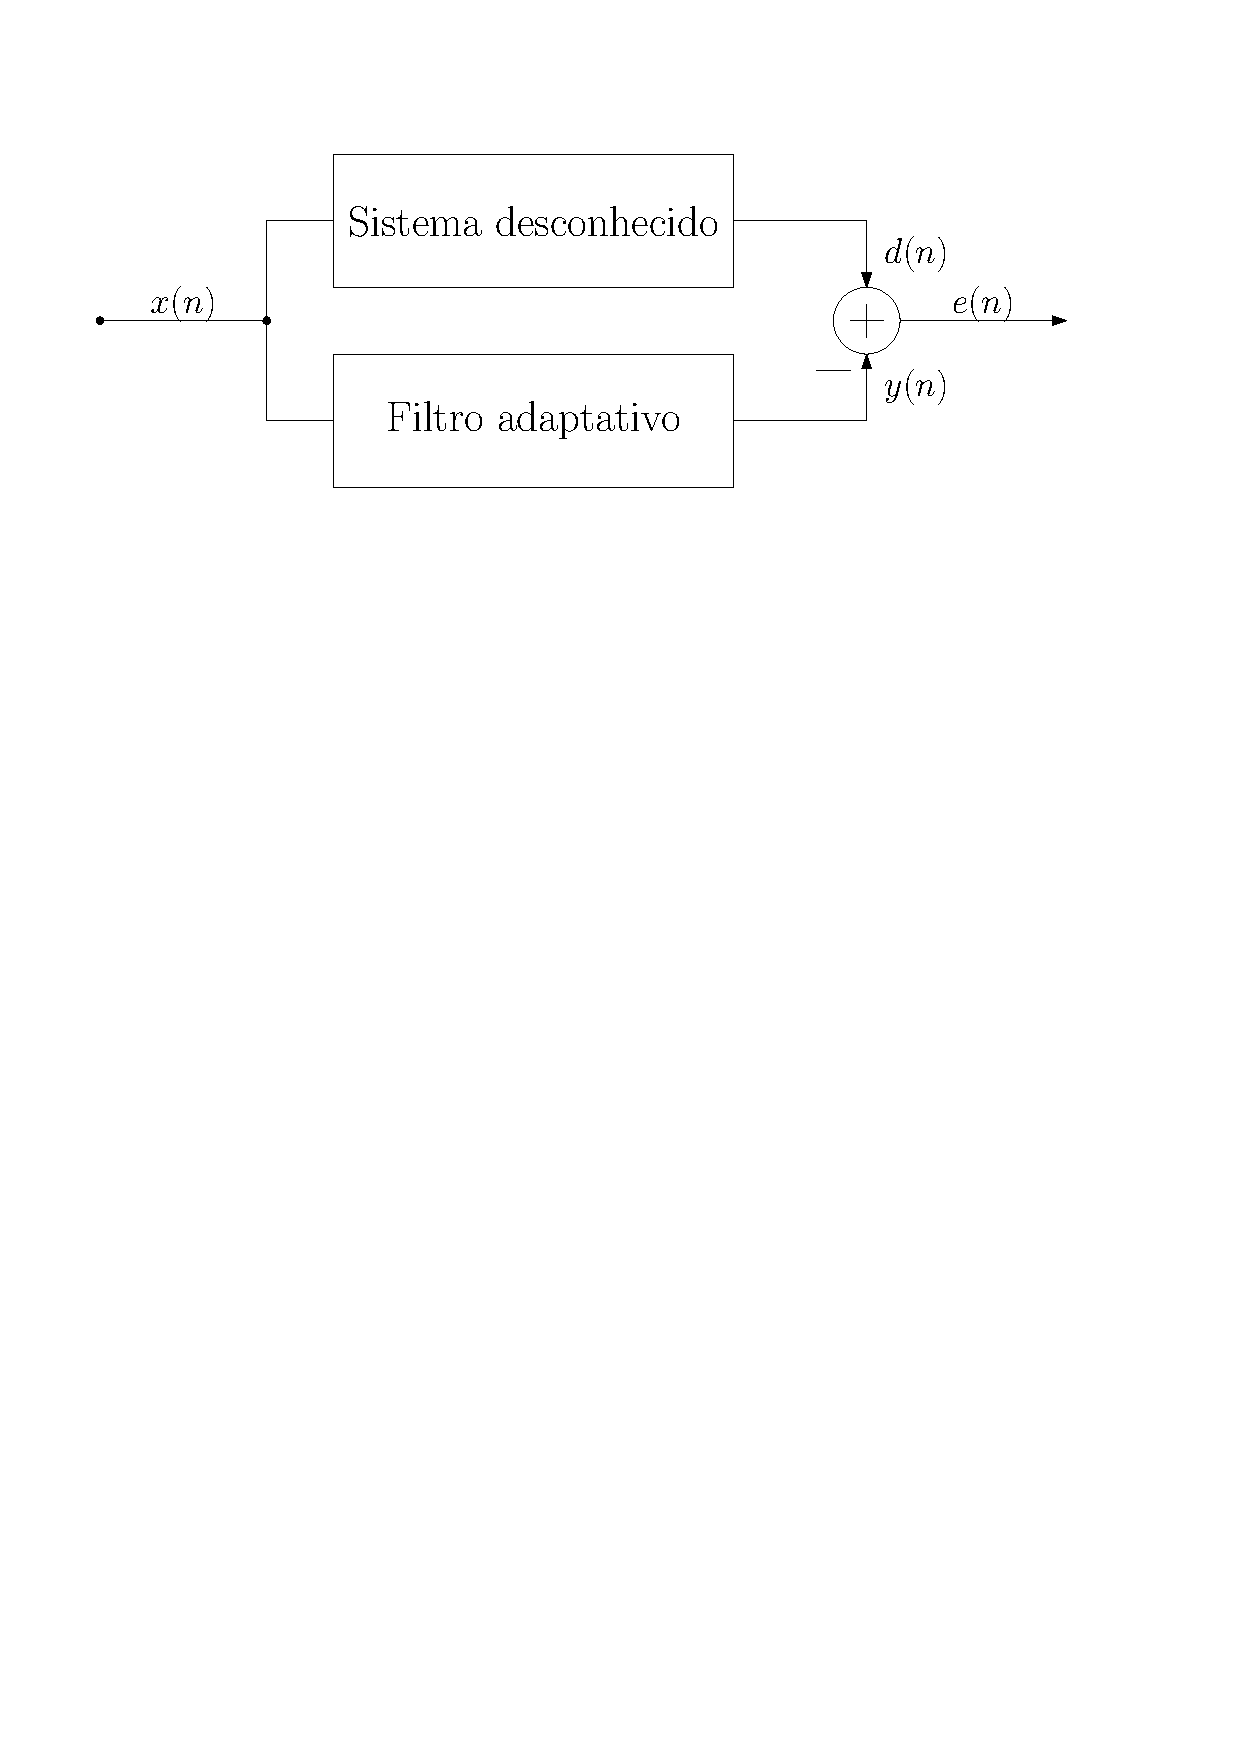
\includegraphics[width=0.6\linewidth]{figs/sistema}
		\caption{Sistema para identificação de sistema.}
		\label{fig:sis}
	\end{figure}

	Neste caso, $x(n)$ é o sinal de entrada, $d(n)$ é o sinal desejado, $y(n)$ é a saída do filtro adaptativo e $e(n)$ é o erro entre a saída do filtro adaptativo e o sinal desejado.
	
	\paragraph{Simulações}
	Primeiro, testei a convergência do algoritmo para diferentes valores de $\lambda$ (ver [1] para conferir a dependência $\lambda$ no algoritmo). Para esta, o sistema desconhecido e o filtro adaptativo tem a mesma ordem. No caso, os dois tem ordem 2. A Figura~\ref{fig:mselms} mostra o MSE (em dB) para diferentes valores de $\mu$. Neste caso foram feitas $50$ rodadas do algoritmo com $800$ iterações cada.
	
	\begin{figure}[!ht]
		\centering
		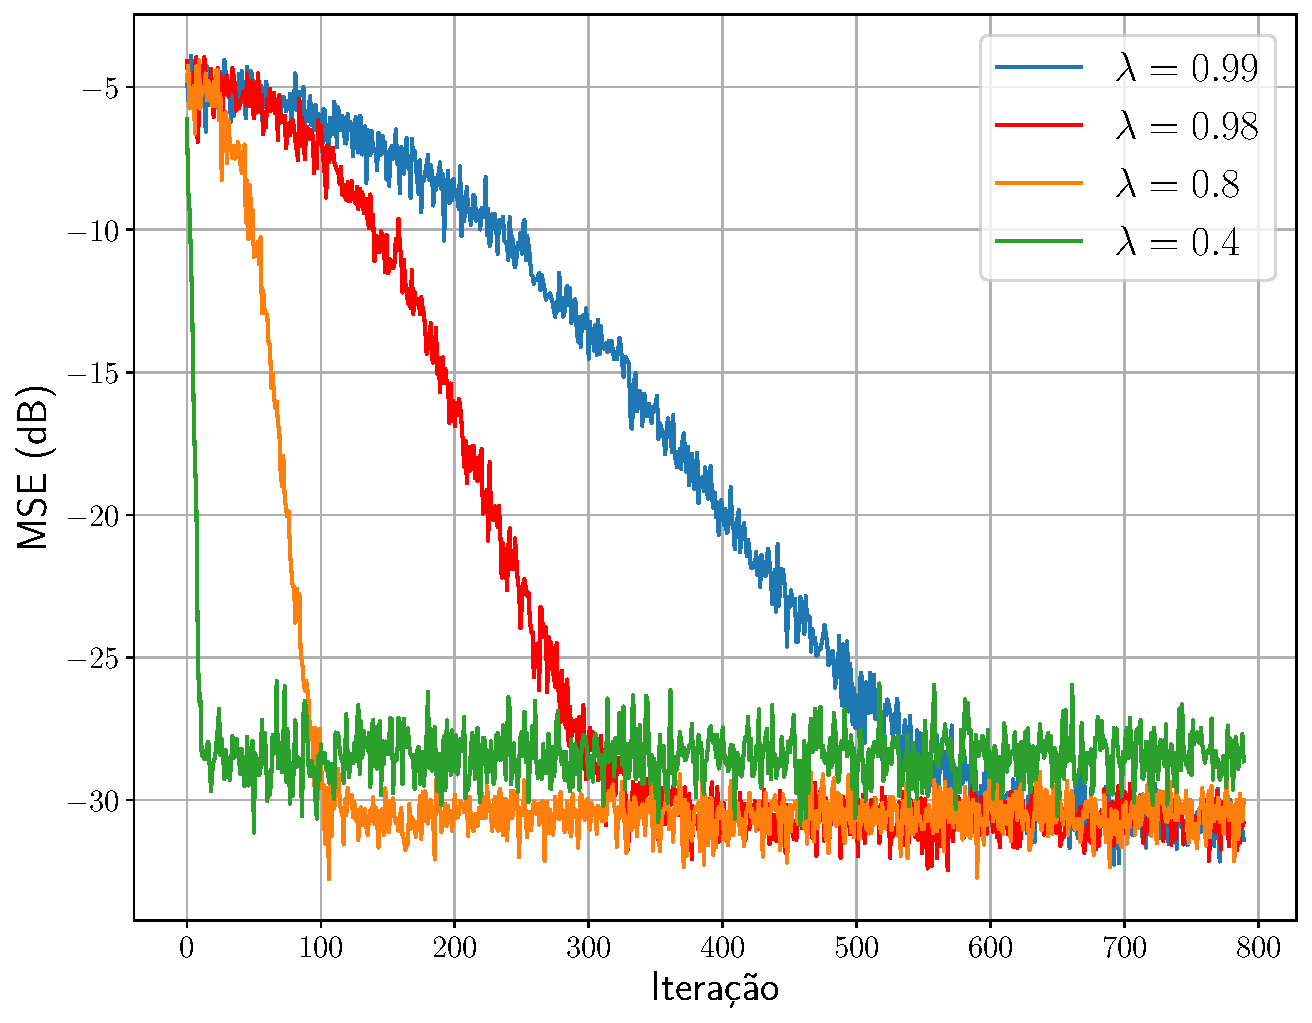
\includegraphics[width=0.75\linewidth]{figs/mse_rls}
		\caption{Curva de MSE (em dB) do algoritmo RLS.}
		\label{fig:mselms}
	\end{figure}
	
	É interessante ver que a pequena mudança entre $\lambda = 0.99$ e $\lambda = 0.98$ faz o algoritmo convergir em muito menos iterações. Também é válido notar o quão rápido, em termos de número de iterações, o algoritmo com $\lambda = 0.4$ converge, mas para um patamar de erro maior do que o dos outros. \\
	
	Agora vamos a convergência dos coeficientes, no caso em que $\lambda = 0.98$ e $\lambda = 0.4$. O coeficientes do sistema a ser identificado são $\wbf_{o}[0] = 0.25$ e $\wbf_{o}[0] = -2$, marcados com uma linha horizontal preta. Na Figura~\ref{fig:coef} temos a evolução a cada iteração dos coeficientes para os $\lambda$ supracitados. Coloquei uma figura bem grande para vermos no detalhe. 
	
	\begin{figure}[!ht]
	\centering
	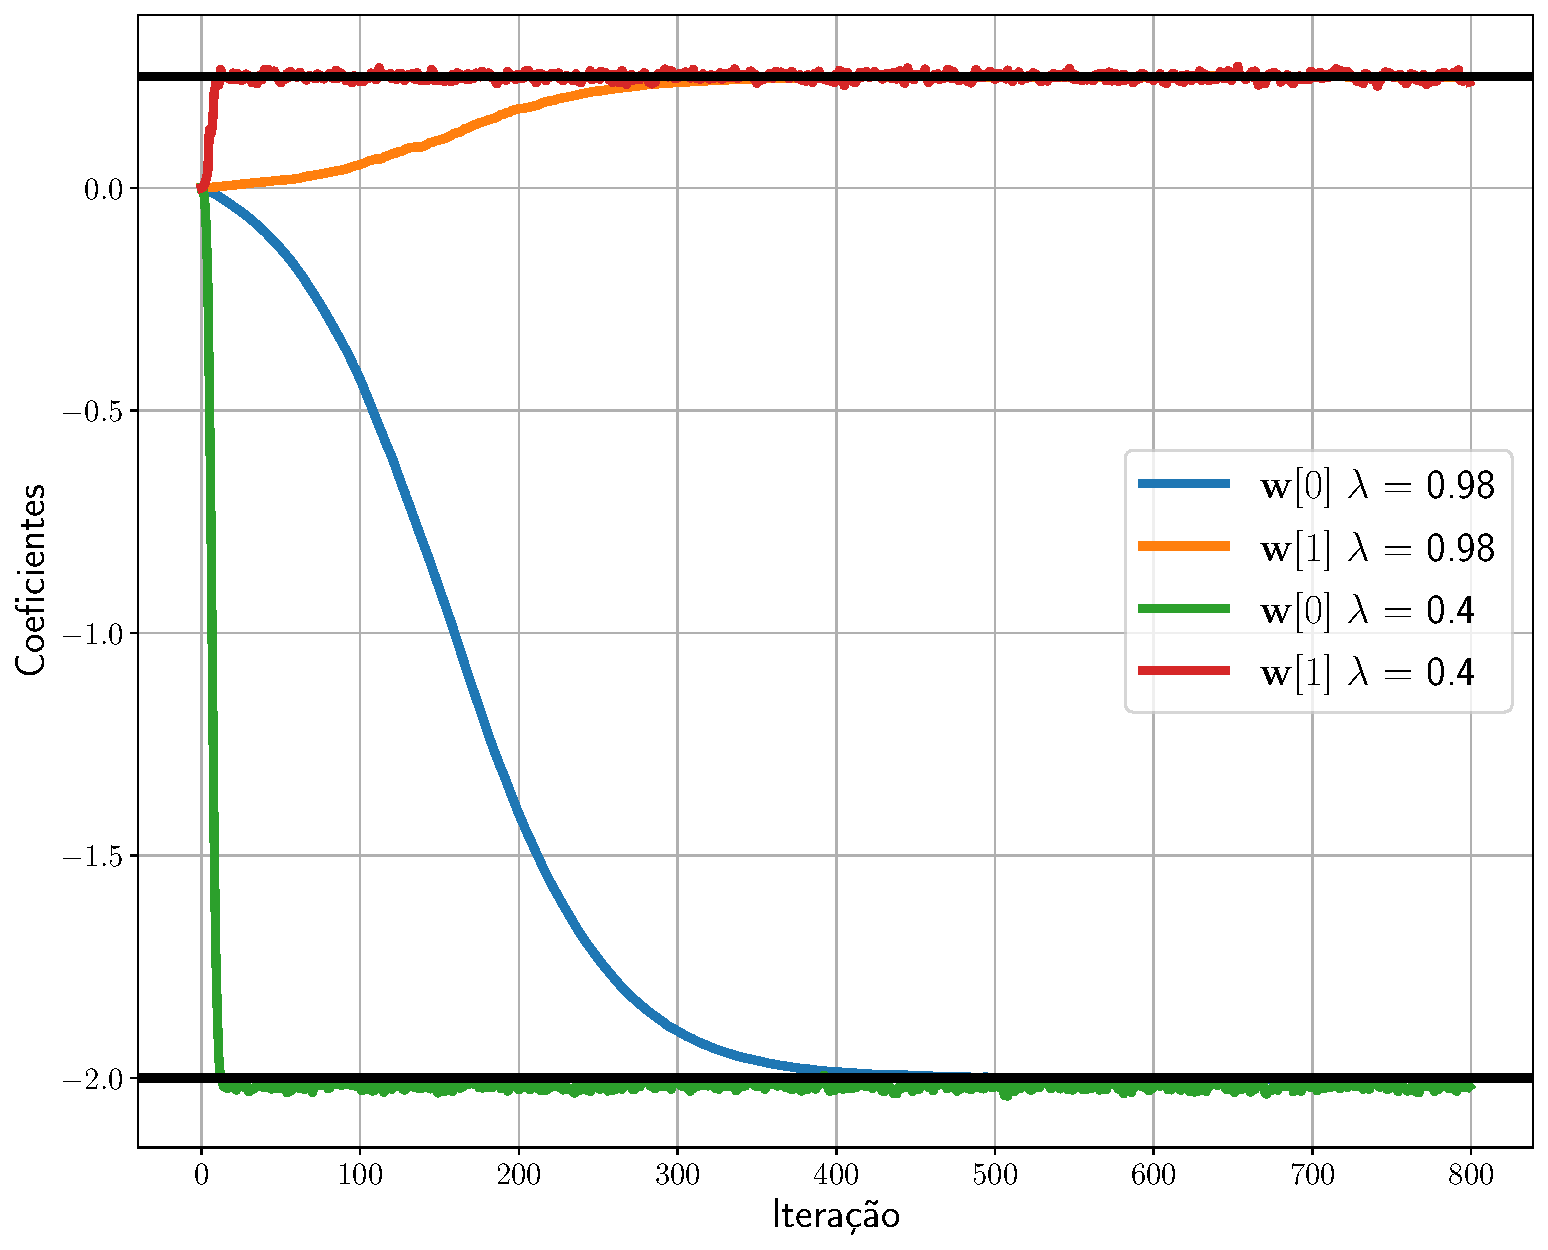
\includegraphics[width=\linewidth]{figs/coeficientes}
	\caption{Variação dos coeficientes do filtro adaptativo.}
	\label{fig:coef}
	\end{figure}
	
	Fica evidente a convergência muito mais rápida para $\lambda = 0.4$, porém com um erro superior em relação ao $\lambda = 0.98$, como já pudia ser visto na figura anterior.
	\pagebreak
	
	Também fiz um teste acrescentando ruído no desejado, como se comporta o RLS. A Figura~\ref{fig:ruido} mostra o comportamento para diferentes valores de $a$, onde $a$ é a amplitude do ruído.
	
	\begin{figure}[!ht]
		\centering
		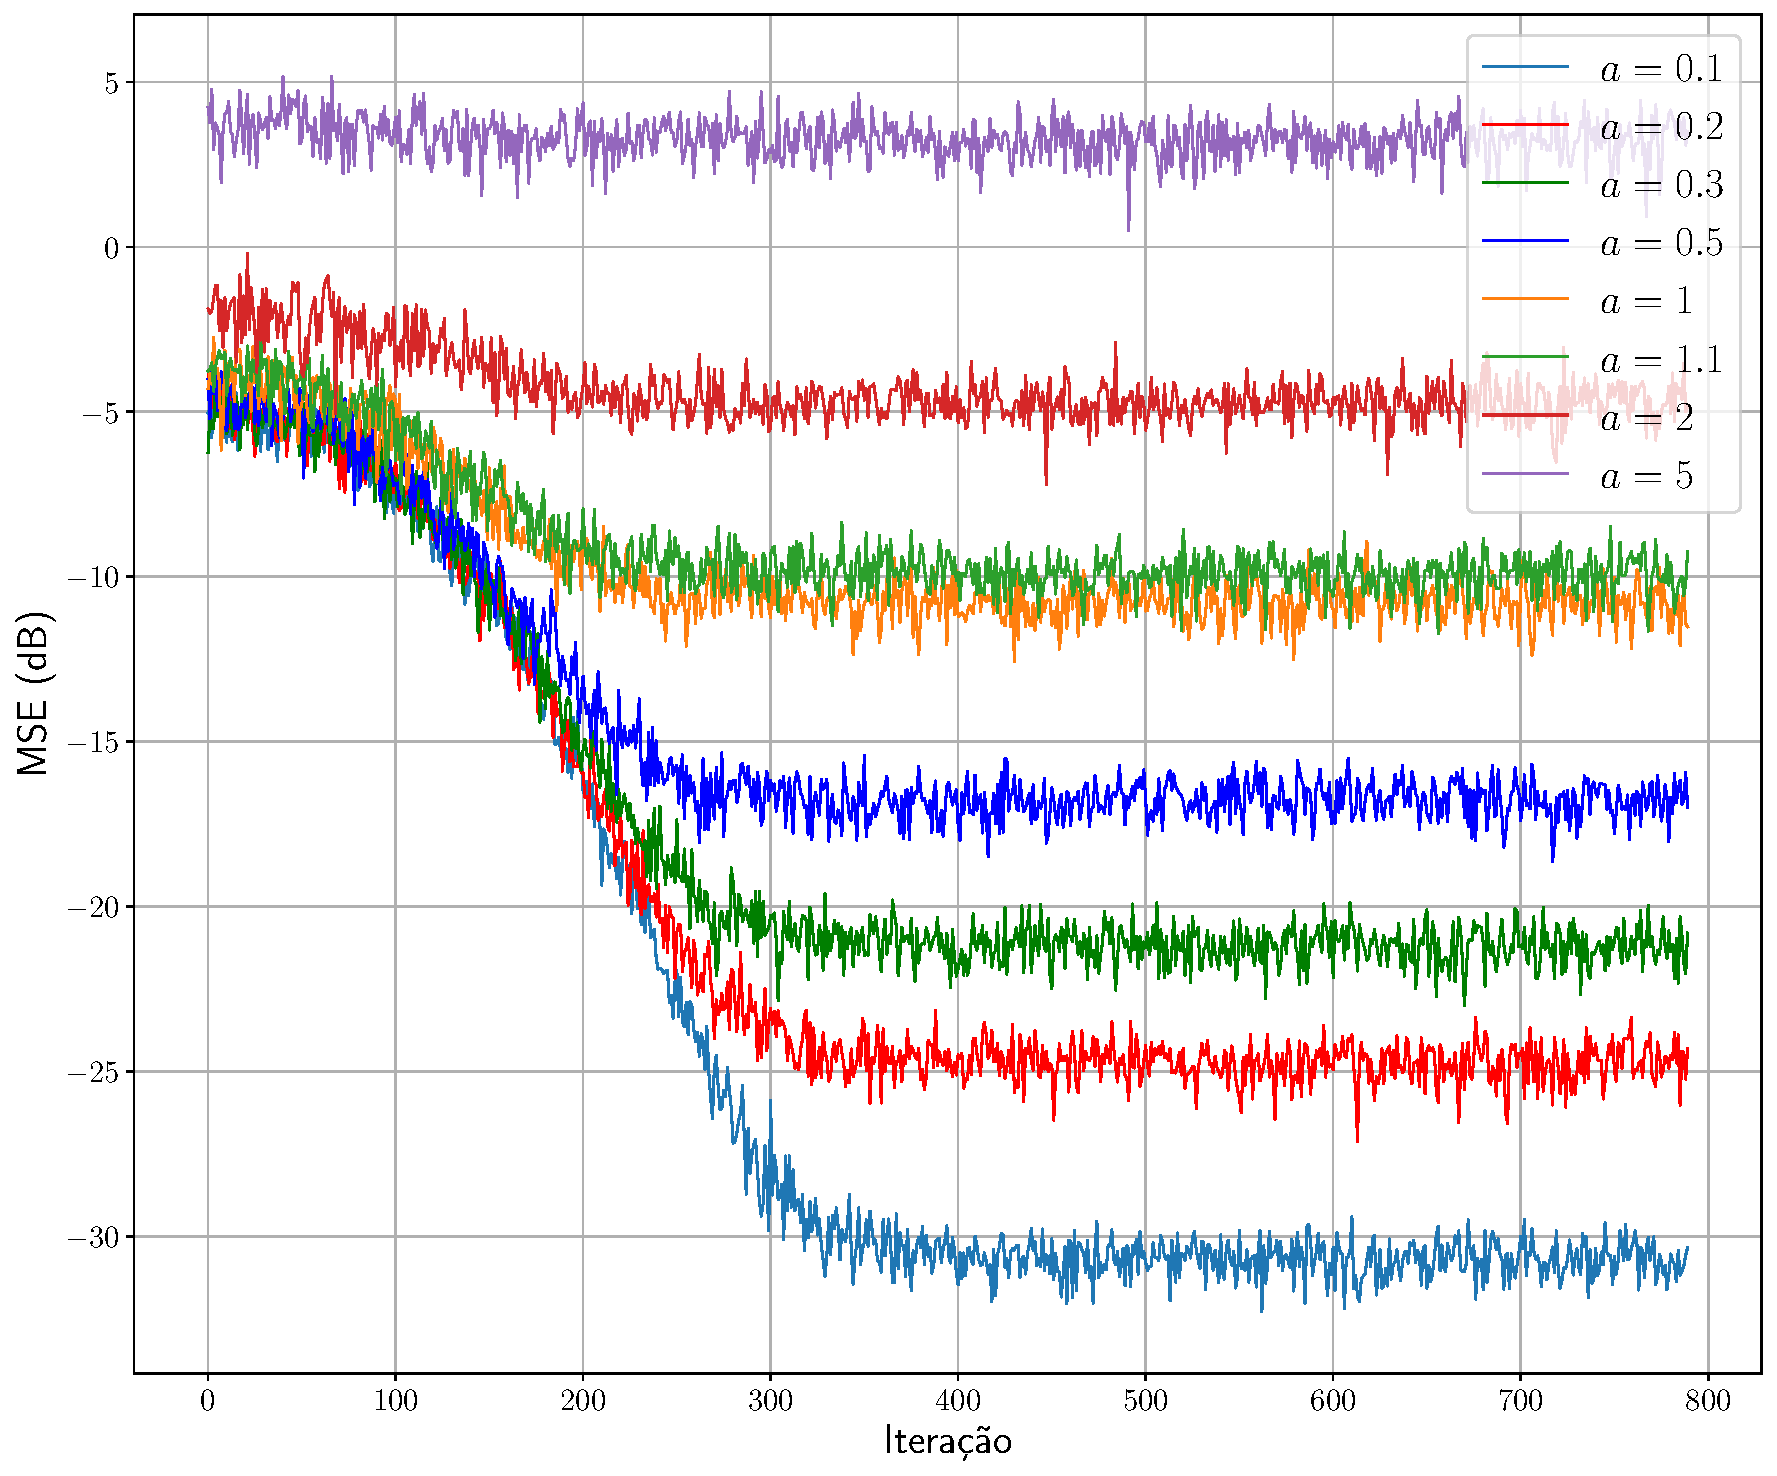
\includegraphics[width=\linewidth]{figs/ruidos}
		\caption{Curvas de MSE (em dB) do algoritmo RLS para diferentes valores de ruído.}
		\label{fig:ruido}
	\end{figure}
	
	Aqui é interessante ver o comportamento do MSE com o acréscimo do ruído, tendo valores de MSE obviamente cada vez maiores para maiores amplitudes do ruído aditivo.
	
\end{homeworkProblem}

\section*{Referências}
[1] P. S. R. Diniz, Adaptive Filtering. Boston, MA: Springer US, 2013.

\end{document}